%!TEX root = ../template.tex
%%%%%%%%%%%%%%%%%%%%%%%%%%%%%%%%%%%%%%%%%%%%%%%%%%%%%%%%%%%%%%%%%%%%
%% chapter2.tex
%% NOVA thesis document file
%%
%% Chapter with the template manual
%%%%%%%%%%%%%%%%%%%%%%%%%%%%%%%%%%%%%%%%%%%%%%%%%%%%%%%%%%%%%%%%%%%%

\typeout{NT FILE chapter2.tex}%

\chapter{Methods}
\label{cha:methods}

\section{System Architecture}

The Prompt2Map system is designed to convert natural language queries into interactive web maps by integrating LLMs with geospatial data retrieval and mapping functionalities. The system architecture comprises two main components: the Geospatial Retriever and the Map Generator. This structure is inspired by the Retrieval-Augmented Generation (RAG) architecture, although it differs in that it retrieves geospatial features instead of documents.

The system workflow involves several key steps. When a user inputs a natural language query expressing their mapping needs, the Geospatial Retriever interprets the query and retrieves relevant geospatial data from the data source. Subsequently, the Map Generator transforms the retrieved data and the user's intent into an interactive web map. Figure \ref{fig:system_logical_architecture} shows this process in detail.


\begin{figure}[htbp]
    \centering
    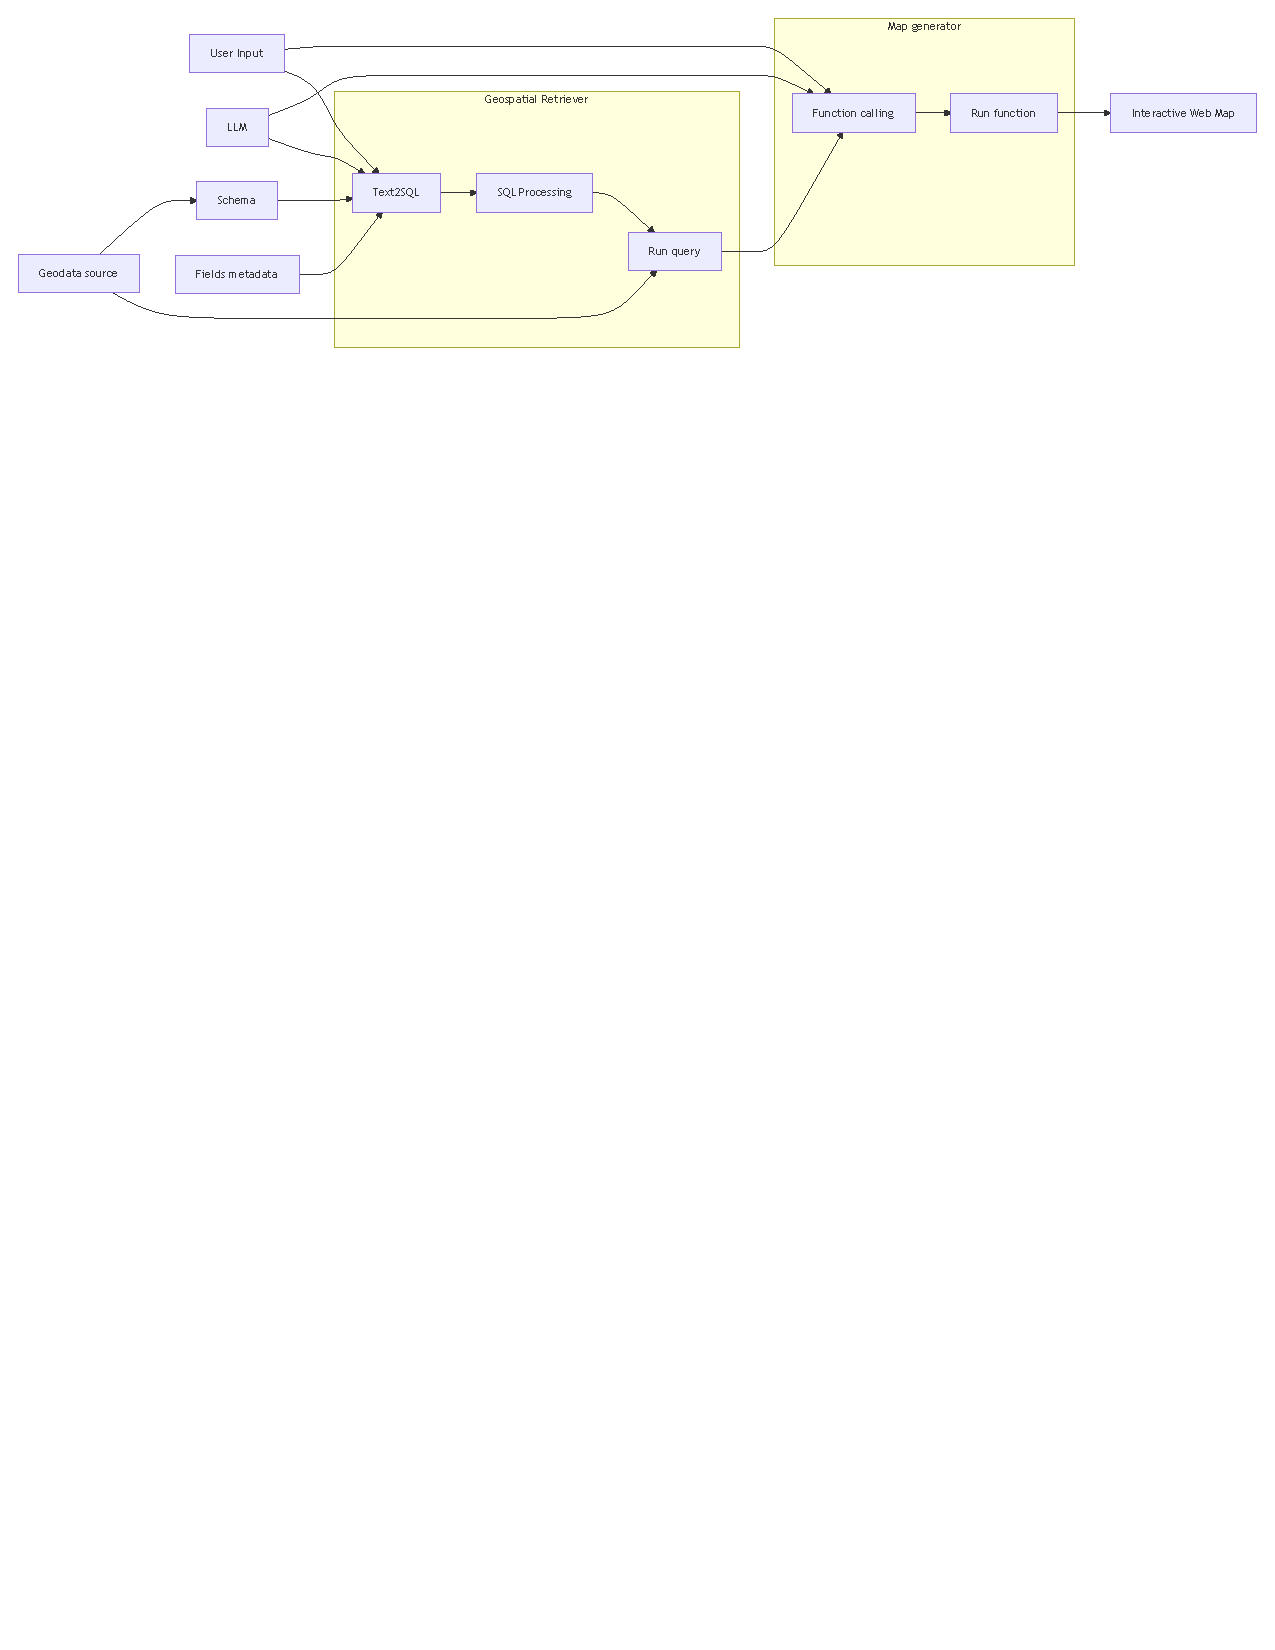
\includegraphics[width=\textwidth]{syscomp}
    \caption{System logical architecture}
    \label{fig:system_logical_architecture}
\end{figure}


\subsection{Geospatial Retriever}

The Geospatial Retriever is responsible for interpreting the user's natural language query and retrieving the relevant geospatial data from the data source. This process involves several subcomponents, including geospatial data sources, text-to-SQL translation, SQL dialect adaptation, SQL processing and validation, and query execution.

\subsubsection{Geospatial Data Sources}

Geospatial data sources constitute the foundation of any GIS application, encompassing a variety of data formats and storage systems that manage the spatial relationships and attributes of features on the Earth's surface. These data sources can take many forms, such as vector and raster datasets, and are stored in specific formats like Shapefiles, GeoPackage, GeoJSON, GeoParquet, and specialized geospatial databases such as PostGIS and DuckDB. Each data source has unique capabilities, optimized for particular types of spatial data, and supports varying levels of data complexity and query functionality. The type of geospatial data source used in a system like Prompt2Map defines the range and complexity of queries that can be performed.

\subsubsection{Text-to-SQL Translation}

As Prompt2Map adopts a RAG-inspired approach, the first step in addressing user queries is to retrieve data relevant to the request. In this context, the target structured language is SQL, which will be executed against DuckDB to query the geospatial data sources. Traditional text-to-SQL models are trained on generic SQL, focusing on "core SQL" keywords like SELECT, GROUP BY, WHERE, etc. Database-specific syntax, such as spatial extensions, are not inherently recognized by these models.

To address this limitation, instead of fine-tuning the model or extensively modifying the prompts to include spatial extensions, the system translates the user query into regular SQL without explicit mentions of geospatial columns. Subsequently, the query is processed to incorporate geospatial features deterministically. This two-step approach ensures that the text-to-SQL translation remains efficient and cost-effective while enabling the integration of spatial functionalities required for accurate data retrieval.

\subsubsection{SQL Processing and Validation}
The generated SQL query undergoes a processing phase that includes validation and correction. Validation involves checking the query for syntactic correctness, security (e.g., preventing SQL injection), and adherence to read-only constraints to protect data integrity. This ensures that the query is safe to execute and will not compromise the underlying database.

Beyond mere validation, the system actively repairs queries by identifying and rectifying potential issues that could lead to incorrect or empty results. For example, if the WHERE clause contains incorrect literals or references nonexistent fields, the system attempts to correct these errors by aligning them with the actual data schema and available metadata. This dual approach of validation and correction enhances the reliability and accuracy of the data retrieval process, ensuring that the resulting datasets are both relevant and correctly structured for subsequent mapping tasks.

After validation, the SQL query is converted to a geospatial DuckDB SQL query by injecting the necessary spatial features. This deterministic modification ensures that the query leverages DuckDB's spatial functions appropriately, enabling accurate and efficient data retrieval based on the user's natural language input.

\subsubsection{Query Execution}
The validated and corrected SQL query is executed against the geospatial data source. The choice of DuckDB as the database engine allows for efficient handling of both single-table and multi-table environments. DuckDB's support for various geospatial data formats and its in-process architecture facilitate seamless data access and manipulation, ensuring that the system can handle a wide range of geospatial queries with high performance.

\subsection{Map Generator}
The Map Generator component transforms the retrieved geospatial data and the user's intent into an interactive web map. This process involves function calling with LLMs, mapping function selection, parameter specification, and map rendering.

\subsubsection{Function Calling with LLMs}
The system utilizes the function-calling feature provided by major LLM API providers, including OpenAI, Claude, and Groq. Function calling allows the LLM to invoke predefined functions with specific parameters based on the user's query and the data characteristics. In this context, the functions correspond to mapping operations, such as generating a choropleth map, a heatmap, or a proportional symbol map. Each function has defined parameters, such as data layers, visual variables, styling options, and interactivity settings.

The LLM analyzes the metadata of the retrieved data, including geometry types, attributes, and spatial relationships. Based on this analysis and the user's intent, the LLM selects the most appropriate mapping function. For example, if the data consists of polygons with quantitative attributes and the user requests to visualize rates or densities, the LLM may select a choropleth mapping function. For point data representing events or occurrences, a heatmap function might be appropriate. Once the mapping function is selected, the LLM specifies the parameters required for the function. These include data layers to be visualized, visual variables to represent attributes through color, size, shape, or texture, styling options like color schemes and classification methods, and interactivity settings such as tooltips, pop-ups, and legends.

The mapping function is executed to render the interactive web map. The system employs web mapping libraries such as Leaflet or Plotly, which support interactive features and responsive design. The final map allows users to interact with the data, providing functionalities like zooming, panning, clicking on features to display attribute information, and toggling layers on and off.

\section{Implementation}

The logical design described in the previous section was implemented as an open-source Python package, available via Python Package Index (PyPI)\footnote{\url{https://pypi.org/project/prompt2map/}} and  Github\footnote{\url{https://github.com/josemcorderoc/prompt2map}}. [Figure @fig:codeimp] shows a Unified Modeling Language (UML) diagram with the project classes and their dependencies.

%![UML class diagram of Prompt2Map implementation in Python](./figs/code_implementation.pdf){#fig:codeimp}

The implementation of Prompt2Map follows a modular architecture, organized into three primary modules: interfaces, providers, and application. This structure adheres to the principles of Clean Architecture, ensuring that the core application logic remains decoupled from external dependencies and infrastructure concerns. Each module serves a distinct purpose within the system, facilitating scalability, maintainability, and ease of integration with various components. In this design paradigm, the application layer is decoupled from the infrastructure layer (providers) by relying on abstract interfaces rather than concrete implementations. 

This approach ensures that the core business logic remains unaffected by changes in external systems or technologies. Specifically, Prompt2Map defines interfaces such as GeoDatabase, Embedding, and LLM within the interfaces module, which outline the essential functionalities required by the application. The providers module contains concrete implementations like GeoDuckDB and OpenAIProvider, which fulfill these interfaces. This modular structure offers significant advantages, including ease of maintenance, scalability, and flexibility. For instance, integrating support for a different geospatial database, such as PostgreSQL with PostGIS, would simply involve creating a new class that implements the GeoDatabase interface without altering the core application logic. This decoupling facilitates adaptability to evolving technological landscapes and simplifies the extension of system capabilities.

Python serves as the primary programming language for implementing Prompt2Map, chosen for its versatility, extensive library support, and strong presence in both the AI and geospatial communities. Python's rich ecosystem includes powerful libraries like GeoPandas, which extends Pandas to enable spatial operations on geospatial data, making it an ideal tool for managing and analyzing geographic information within the system.

\subsection{Application}
The application component constitutes the core functionality of the prompt2map package, orchestrating the end-to-end process of converting natural language queries into interactive web maps. This component is responsible for managing the workflow from query interpretation to data retrieval and finally to map generation. By leveraging the abstract interfaces defined within the interfaces module and utilizing the concrete implementations provided by the providers, the application layer ensures seamless interaction between different system modules. This modular approach not only enhances the system's scalability but also facilitates easier maintenance and future enhancements.

Within the application component, key classes such as `SQLGeoRetriever`, `LLMPrompt2SQL`, `LLMMapGenerator`, and `Prompt2Map` play pivotal roles. `SQLGeoRetriever` handles the translation of natural language queries into SQL statements and manages the retrieval of geospatial data from the database. `LLMPrompt2SQL` utilizes the capabilities of LLMs to accurately convert user prompts into executable SQL queries, ensuring that the data retrieval process aligns with the user's intent. `LLMMapGenerator` is tasked with transforming the retrieved geospatial data into visually coherent and interactive maps, selecting appropriate visualization techniques based on the nature of the data and the user's requirements. Finally, the `Prompt2Map` class serves as the primary interface for users, integrating the functionalities of the retriever and generator to deliver a cohesive mapping experience. This structured separation of responsibilities within the application component ensures that each aspect of the system operates efficiently and cohesively.

\subsection{Interfaces}
The interfaces component serves as the foundational layer of the prompt2map package, defining the abstract contracts that dictate how different modules interact with one another. By establishing clear and standardized interfaces, the system ensures that each component adheres to a consistent set of functionalities, promoting interoperability and flexibility. This abstraction is crucial for maintaining a decoupled architecture, allowing individual modules to be developed, tested, and maintained independently without impacting the overall system integrity.

Key interfaces within this component include `Embedding`, `LLM`, `GeoDatabase`, `GeoRetriever`, `Prompt2SQL`, and `MapGenerator`. The `Embedding` interface outlines the methods required for generating numerical representations of textual data, which are essential for tasks like similarity matching and query understanding. The `LLM` interface defines the interaction methods with LLMs, facilitating tasks such as prompt-based query generation and response handling. `GeoDatabase` encapsulates the functionalities needed to interact with geospatial databases, including schema retrieval and geospatial data querying. `GeoRetriever` specifies the methods for fetching geospatial data based on user queries, ensuring that the application can retrieve relevant and accurate datasets. `Prompt2SQL` bridges the gap between natural language inputs and structured SQL queries, enabling the seamless translation of user intents into executable database commands. Lastly, the `MapGenerator` interface outlines the methods for creating interactive maps from geospatial data, ensuring that visualizations are generated consistently and effectively. By defining these interfaces, the system promotes a high level of abstraction and modularity, allowing for easy integration of new functionalities and technologies as the system evolves.

\subsection{Providers}
The providers component encapsulates the concrete implementations of the abstract interfaces defined within the interfaces module. This layer is responsible for managing interactions with external services and tools, effectively bridging the gap between the system's core functionalities and the underlying technologies that enable them. By centralizing these implementations within the providers, the system achieves a high degree of flexibility and adaptability, allowing for seamless integration of new services or replacement of existing ones without disrupting the core application logic.

Within the providers module, classes such as `GeoDuckDB` and `OpenAIProvider` play critical roles. `GeoDuckDB` implements the `GeoDatabase` interface, managing all interactions with DuckDB, the chosen geospatial database engine. This includes handling data storage, executing spatial queries, and managing database connections. DuckDB's in-process architecture and robust support for various geospatial data formats make it an ideal choice for efficient data retrieval and management within Prompt2Map. On the other hand, `OpenAIProvider` implements both the `LLM` and `Embedding` interfaces, facilitating interactions with the OpenAI API. This provider manages the communication with LLMs, enabling the system to leverage advanced natural language processing capabilities for tasks such as text-to-SQL translation and function calling. By abstracting these external dependencies into dedicated provider classes, the system ensures that changes or updates to external services can be accommodated with minimal impact on the overall architecture. Additionally, this separation of concerns enhances the maintainability and scalability of the system, allowing developers to focus on core functionalities without being bogged down by the complexities of external service integrations.

\subsection{External Dependencies}
The prompt2map package leverages several external dependencies to achieve its functionality, each chosen for its robustness, performance, and compatibility with the system's requirements.

\subsubsection{OpenAI API}
The OpenAI API is integrated into Prompt2Map to leverage the advanced natural language processing capabilities of LLMs like GPT-4. This API facilitates the system's ability to interpret and translate natural language queries into executable SQL statements through the text-to-SQL functionality. By utilizing the OpenAI API, Prompt2Map can effectively handle complex and nuanced user inputs, ensuring accurate data retrieval and meaningful map generation. The API provides access to powerful language models that excel in understanding context, disambiguating meanings, and generating coherent and contextually relevant responses. Additionally, the OpenAI API supports function calling, allowing Prompt2Map to invoke predefined mapping functions with specific parameters based on user queries. This integration enhances the system's ability to maintain consistency and standardization in map generation, as the predefined functions ensure that all maps adhere to established cartographic principles and visualization standards. Moreover, the use of the OpenAI API abstracts the complexities of managing and deploying LLMs, enabling Prompt2Map to focus on delivering a seamless and user-friendly GIS experience without the overhead of maintaining sophisticated NLP infrastructure.


\subsubsection{DuckDB}
DuckDB is employed as the primary geospatial database engine within Prompt2Map, selected for its high performance, in-process architecture \cite{raasveldt_duckdb_2019},  and comprehensive support for geospatial data types and functions. Unlike traditional SQL databases that require separate server infrastructure, DuckDB operates entirely within the application's process, eliminating the need for additional setup and reducing latency in data retrieval. Its geospatial extension provides robust capabilities for handling spatial queries, including spatial joins, proximity searches, and geographic aggregations, which are essential for generating accurate and informative maps. DuckDB's ability to efficiently manage large datasets and perform complex queries makes it an ideal choice for Prompt2Map, ensuring swift data processing and reliable performance. Furthermore, DuckDB''s compatibility with various geospatial data formats, such as GeoJSON, Shapefiles, and GeoParquet, enhances the system's flexibility and ease of data integration, allowing Prompt2Map to seamlessly incorporate diverse geospatial datasets without compromising on performance or functionality.


\section{Data}
The Prompt2Map system is designed to work with various structured spatial data sources. For this thesis, we use the Portuguese 2021 Census Data. This dataset includes demographic, socioeconomic and housing information structured in a single-table format, suitable for testing basic SQL queries and simple map visualizations. The data attributes encompass population counts (total population, age groups), socioeconomic indicators (employment rates, education levels, household income), and geographic units (administrative boundaries at different levels, such as municipalities and regions). The data is obtained from the Portuguese National Statistics Institute (INE) \cite{INE2021Census}.

\section{Evaluation}

% Paragraph 1: The challenges of measuring the performance of Prompt2Map

Evaluating the performance of Prompt2Map poses several challenges due to the system's unique characteristics, including the integration of natural language processing, geospatial data retrieval, and map generation functionalities. Traditional evaluation metrics used in NLP, such as BLEU scores or F1 scores, may not fully capture the system's effectiveness in converting natural language queries into interactive web maps. Therefore, a comprehensive evaluation strategy is required to assess the system's performance across different dimensions, including accuracy, efficiency, usability, and scalability.

% Paragraph 2: Say that for the scope of this thesis, we focus on the text-to-SQL evaluation (this is, the retriever), as the mapping evaluation is more subjective. And also the map is generated basically by the webmap libraries

Nevertheless, for the scope of this thesis, the evaluation focuses on the text-to-SQL translation component of Prompt2Map, which corresponds to the Geospatial Retriever in the system architecture. This evaluation aims to assess the system's ability to accurately interpret natural language queries, generate SQL statements that retrieve relevant geospatial data, and execute these queries against the geospatial database. The evaluation of the Map Generator component, which involves the creation of interactive web maps based on the retrieved geospatial data, is more subjective and user-dependent, making it challenging to define objective metrics. Therefore, the focus of this evaluation is on the Geospatial Retriever, which forms the foundation of the system's functionality.

% TODO: Question table
\subsection{Metrics}

\subsubsection{The problem with text-to-SQL metrics}

Can a question be represented as a SQL query? This is the main question that text-to-SQL systems aim to answer. However, evaluating the performance of these systems is challenging due to the inherent ambiguity and complexity of natural language queries. Even for human annotators, determining the correct SQL query for a given question can be a non-trivial task, as it requires an understanding of the underlying database schema, the semantics of the question, and the intended query result. Therefore, developing robust evaluation metrics that can accurately assess the performance of text-to-SQL systems is crucial for advancing the field and enabling fair comparisons between different approaches.

There are multiple benchmarks for text-to-SQL evaluation, such as Spider \cite{yu_spider_2018}, BIRD \cite{li_can_2023} and WikiSQL \cite{zhongSeq2SQL2017}. These benchmarks provide standardized datasets with natural language questions paired with their corresponding SQL queries, allowing researchers to evaluate the performance of their systems on common tasks. The two main evaluation metrics for the text-to-SQL task are Exact Matching (EM) and Execution Accuracy (EX), introduced by Spider. EM measures the syntax-level equivalence between the generated SQL query and the ground truth query, while EX evaluates the execution results of the generated query.

\begin{equation}
    \text{EM} = \frac{\text{Number of exact matches}}{\text{Total number of queries}}
\end{equation}

\begin{equation}
    \text{EA} = \frac{\text{Number of correct executions}}{\text{Total number of queries}}
\end{equation}


However, those metrics have limitations that can lead to biased results and inaccurate performance assessments \cite{kim_flex_2024}. While EM evaluates the syntax-level equivalence of queries, it often leads to high false negative rates, as the same logical intent can be represented through various query structures and alises. On the other hand, EX focuses on the execution results of the generated queries, providing a more robust evaluation metric. However, EX is not without its limitations, as it can produce false positives when incorrect queries yield correct results, and false negatives when extra fields are included in the output.

\subsubsection{Soft F1-Score}

The hardness of EM and EX is that both require exact matches between the generated SQL query and the ground truth. This is a very strict requirement, as even small variations in the generated query can lead to a mismatch. To address this issue, the Soft F1-score was introduced as a more lenient evaluation metric that considers the data similarity between the generated and ground truth queries. 

The original F1-score is a metric commonly used in classification tasks to balance the model's ability to correctly identify positive samples (precision) and to capture all positive samples (recall). 

Precision is the proportion of true positive samples out of the total number of samples predicted as positive. It evaluates the model's accuracy in identifying positive samples (Equation \ref{eq:precision}). Recall is the proportion of true positive samples out of the total number of positive samples in the dataset. It measures the model's ability to capture all positive samples (Equation \ref{eq:recall}). The F1-score is the harmonic mean of precision and recall, providing a balanced evaluation metric that considers both aspects of the model's performance (Equation \ref{eq:f1}).

\begin{equation}
    \text{Precision} = \frac{\text{True Positives}}{\text{True Positives} + \text{False Positives}}
    \label{eq:precision}
\end{equation}

\begin{equation}
    \text{Recall} = \frac{\text{True Positives}}{\text{True Positives} + \text{False Negatives}}
    \label{eq:recall}
\end{equation}

\begin{equation}
    \text{F1} = 2 \times \frac{\text{Precision} \times \text{Recall}}{\text{Precision} + \text{Recall}}
    \label{eq:f1}
\end{equation}

In the context of text-to-SQL evaluation, the definition of what is a true/false positive/negative is what differences the metrics. EM considers a true positive when the generated query is exactly the same as the ground truth. EX considers a true positive when the generated query returns the exact same results as the ground truth. The Soft F1-score relaxes the requirement of exact matches, considering the similarity between the generated and ground truth queries, as shown in Figure \ref{fig:tp_tn_sql}.

\begin{figure}[htbp]
    \centering
    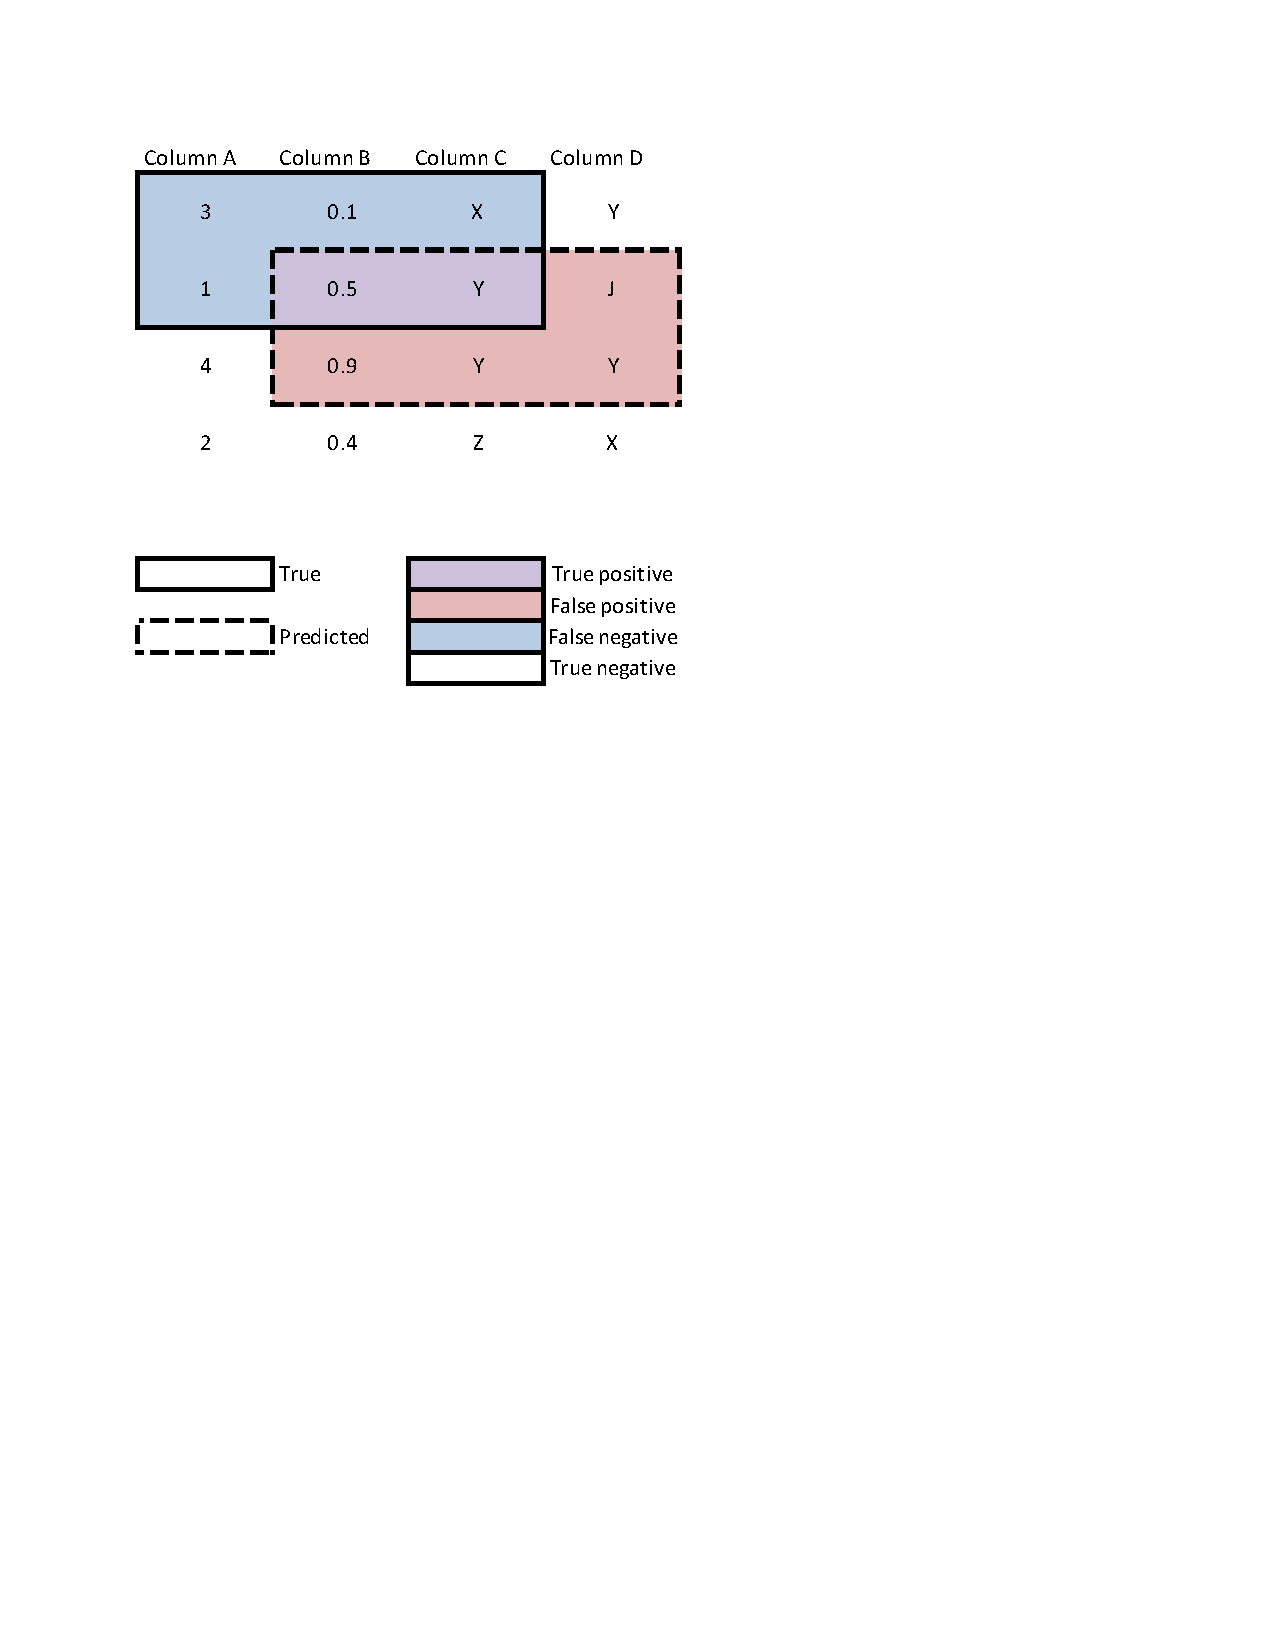
\includegraphics[width=0.5\textwidth]{tp_tn_sql}
    \caption{True and False Positives and Negatives in SQL evaluation for Soft F1-score. The solid border represents the ground truth, while the dashed border represents the generated query.}
    \label{fig:tp_tn_sql}
\end{figure}

\subsubsection{Consistency}

To assess the consistency of the Prompt2Map outputs across multiple runs, we introduced a metric termed Consistency Entropy. The entropy (Equation \ref{eq:entropy}) is the amount of bits required to encode the information in a message, and it is a measure of uncertainty. The normalized entropy (Equation \ref{eq:norm_entropy}) is the entropy divided by the maximum possible entropy, which is the logarithm of the number of possible outputs. This normalization ensures that the entropy value is between 0 and 1, making it comparable across different scenarios. The Consistency Entropy (Equation \ref{eq:consistency_entropy}) is defined as \(1 - \text{normalized entropy}\), where a higher score indicates higher consistency.

\begin{equation}
    H(X) = - \sum_{i=1}^{n} p(x_i) \log_2 p(x_i)
    \label{eq:entropy}
\end{equation}

\begin{equation}
    H_{rel}(X) = \frac{H(X)}{\log_2 n} 
    \label{eq:norm_entropy}
\end{equation}

\begin{equation}
    \text{Consistency Entropy} = 1 - H_{rel}(X)
    \label{eq:consistency_entropy}
\end{equation}


%a measure of uncertainty, or of "poorness of a guess," which will be high when the number of alternative possibilities is nigh, and low when some of the possibilities are much more likely than others

For example, consider two different output distributions for a given prompt. If the system consistently generates the same output "AAAAA" across all runs, the entropy of this distribution is zero, indicating no uncertainty, and the consistency score is 1, reflecting perfect consistency. Conversely, if the system produces a uniform distribution of outputs "A", "B", "C", "D", and "E" with equal probability, the entropy reaches its maximum value, indicating high uncertainty, and the consistency score is minimized, reflecting low consistency.

This might lead to cases that are unintuitive. For instance, the normalized entropy of AAAAABBBBB is the same as ABCDEFGHIJ (both are 1), but the second one has more diversity. This is because the normalized entropy is compares the distribution of the outputs, not the outputs themselves. Both ouputs are uniformly distributed, there for the same normalized entropy (the maximum value).

As diversity is also a relevant aspect of the system's performance, we introduce a second metric, the relative mode frequency (Equation \ref{eq:mode_frequency}). This metric provides a simple yet effective measure of the most common output generated by the system across multiple runs. A high mode frequency indicates that the system consistently produces a specific output, which can be beneficial for tasks requiring deterministic results. By combining Consistency Entropy and mode frequency, the evaluation framework captures both the diversity and stability of the system's outputs, offering a comprehensive assessment of its performance.

\begin{equation}
    \text{Mode Frequency (X)} = \frac{\text{Number of occurrences of the mode}}{\text{Total number of runs}} = \frac{\max_{x \in X} \text{count}(x)}{|X|}
    \label{eq:mode_frequency}
\end{equation}


This metric penalizes having a high diversity of outputs. For example, the relative mode frequency of AAAAABBBBB is $\frac{1}{2}$, while the relative mode frequency of ABCDEFGHIJ is 0.1. This metric complements the Consistency Entropy by providing a measure of the most common output generated by the system, offering insights into the system's deterministic behavior.


\subsection{Evaluation Questions}

The metrics presented in the previous section are used to evaluate the performance of the Prompt2Map system across a series of evaluation questions. These questions are designed to test the system's ability to accurately interpret natural language queries, generate SQL statements that retrieve relevant geospatial data, and execute these queries against the geospatial database. By evaluating the system's performance on a diverse set of queries, we can assess its effectiveness in handling various types of user inputs and producing accurate and informative maps.

Each question is accompanied by the expected SQL query, which serves as the ground truth for evaluating the system's performance. The evaluation questions are designed to test the system's ability to handle different types of queries, including aggregation, filtering, and spatial analysis tasks. By evaluating the system's performance on these questions, we can gain insights into its strengths and limitations, identify areas for improvement, and guide future development efforts.

{\scriptsize

\definecolor{dkgreen}{rgb}{0,0.6,0}
\definecolor{gray}{rgb}{0.5,0.5,0.5}
\definecolor{mauve}{rgb}{0.58,0,0.82}

\lstset{
  language=SQL,
  basicstyle=\ttfamily\scriptsize, % set font size to small
  keywordstyle=\color{blue},
  commentstyle=\color{dkgreen},
  stringstyle=\color{mauve},
  numbers=none,
  frame=none,
  showstringspaces=false,
  columns=flexible,
  breaklines=true
}

\bgroup
\rowcolors{1}{}{GhostWhite}
\begin{xltabular}{\textwidth}{|p{0.05\textwidth}p{0.3\textwidth}p{0.55\textwidth}|}
    \caption{Evaluation questions for the Prompt2Map system.}
    \label{tab:evaluation_questions}\\
    \toprule
    \rowcolor{Gainsboro}%
       ID & Question & Expected SQL \\
    \midrule
\phantomsection\label{question:1}Q1 & Which Freguesias have the highest percentage of buildings constructed before 1945? & \lstinline!SELECT c.Freguesia, (c.N_EDIFICIOS_CONSTR_ANTES_1919 + c.N_EDIFICIOS_CONSTR_1919A1945) / (c.N_EDIFICIOS_CLASSICOS) * 100 AS percentage, c.geometry FROM censo2021pt.censo2021_freguesia c ORDER BY percentage DESC;! \\
\phantomsection\label{question:2}Q2 & How does the absolute distribution of one- or two-floor buildings vary across Municipios? & \lstinline!SELECT c.Municipio, SUM(c.N_EDIFICIOS_1OU2_PISOS) AS building_count, ST_Union(c.geometry) AS geometry FROM censo2021pt.censo2021_freguesia c GROUP BY c.Municipio;! \\
\phantomsection\label{question:3}Q3 & In which Distritos is the absolute number of single-family or two-family homes highest? & \lstinline!SELECT c.Distrito, SUM(c.N_EDIFICIOS_CLASSICOS_1OU2_ALOJ) AS single_family_homes, ST_Union(c.geometry) AS geometry FROM censo2021pt.censo2021_freguesia c GROUP BY c.Distrito ORDER BY single_family_homes DESC;! \\
\phantomsection\label{question:4}Q4 & What is the ratio of rented housing to owned housing in different Freguesias? & \lstinline!SELECT c.Freguesia, (c.N_RHABITUAL_ARRENDADOS) / (c.N_RHABITUAL_PROP_OCUP) AS rent_own_ratio, c.geometry FROM censo2021pt.censo2021_freguesia c ORDER BY rent_own_ratio DESC;! \\
\phantomsection\label{question:5}Q5 & What percentage of buildings are constructed with three or more apartments in each Freguesia? & \lstinline!SELECT c.Freguesia, (c.N_EDIFICIOS_CLASSICOS_3OUMAIS\_ALOJ / c.N_EDIFICIOS_CLASSICOS) * 100 AS multi_family_density, c.geometry FROM censo2021pt.censo2021_freguesia c ORDER BY multi_family_density DESC;! \\
\phantomsection\label{question:6}Q6 & Which Municipios have the highest proportion of individuals aged 65 or older? & \lstinline!SELECT c.Municipio, SUM(c.N_INDIVIDUOS_65_OU_MAIS) / SUM(c.N_INDIVIDUOS) * 100 AS age_65_plus_percentage, ST_Union(c.geometry) AS geometry FROM censo2021pt.censo2021_freguesia c GROUP BY c.Municipio ORDER BY age_65_plus_percentage DESC;! \\
\phantomsection\label{question:7}Q7 & Which Freguesias have the highest male-to-female ratio in the population? & \lstinline!SELECT c.Freguesia, (c.N_INDIVIDUOS_H / NULLIF(c.N_INDIVIDUOS_M, 0)) AS male_to_female_ratio, c.geometry FROM censo2021pt.censo2021_freguesia c ORDER BY male_to_female_ratio DESC;! \\
\phantomsection\label{question:8}Q8 & Where are parking-accessible residential accommodations more common across Municipios relative to all residences? & \lstinline!SELECT c.Municipio, SUM(c.N_RHABITUAL_COM_ESTACIONAMENTO) / SUM(c.N_CLASSICOS_RES_HABITUAL) * 100 AS parking_accessible, ST_Union(c.geometry) AS geometry FROM censo2021pt.censo2021_freguesia c GROUP BY c.Municipio ORDER BY parking_accessible DESC;! \\
\phantomsection\label{question:9}Q9 & What is the percentage of individuals with no formal education across Distritos? & \lstinline!SELECT c.Distrito, SUM(c.N_INDIVIDUO_ENSINCOMP_NENHUM) / SUM(c.N_INDIVIDUOS) * 100 AS no_education_percentage, ST_Union(c.geometry) AS geometry FROM censo2021pt.censo2021_freguesia c GROUP BY c.Distrito ORDER BY no_education_percentage DESC;! \\
\phantomsection\label{question:10}Q10 & In which Freguesias is the unemployment rate highest? & \lstinline!SELECT c.Freguesia, ((c.N_INDIVIDUOS_DESEMPREGADOS_1EMP + c.N_INDIVIDUOS_DESEMPREGADOS_NOVOEMP) / NULLIF(c.N_INDIVIDUOS_COM_ATIVIDADE_ECONOMICA, 0)) * 100 AS unemployment_rate, c.geometry FROM censo2021pt.censo2021_freguesia c ORDER BY unemployment_rate DESC;! \\
    \bottomrule
\end{xltabular}
\egroup
}

% hyperref[question:10]{Question 10}
\subsection{Aggregation}

All the questions were tested 10 times using the prompt2map package. For each test, the system generated a SQL query based on the natural language question, which was used to compute the previously described metrics. The 10 results were aggregated as it follows:

\begin{itemize}
       \item Completion rate: percentage of successful completions (i.e., the system generated a valid SQL query that executed without errors) out of the total number of runs.
       \item Macro Precision: the average precision across all runs.
       \item Macro Recall: the average recall across all runs.
       \item Macro Soft F1-score: the average Soft F1-score across all runs.
       \item Frequency of the mode: the frequency of the most common output generated by the system across all runs.
       \item Consistency Entropy: the normalized entropy of the model's output distribution across all runs.
\end{itemize}
   